\chapter{Results}\label{chapter_sta}
Throughout previous chapters I have provided the motivation for my exploratory study that investigates the possibility of recurrent behaviors discovery from software process artifacts; discussed the previous work in the research field of software repository mining, identifying unexplored and underexplored directions; and proposed a novel data-mining technique, which, potentially, can automate the discovery of recurrent behaviors from software process artifacts measurements.

In this chapter, I shall present, evaluate, and discuss \mbox{SAX-VSM}-based implementation of the Software Trajectory Analysis  framework (STA) that provides end-to-end generic and customizable workflow for recurrent behaviors discovery from Software Trajectories, that are ordered sequences of software artifact measurements. 
As I shall show in this Chapter, throughout my exploratory study, STA has evolved from a narrow focused tool to a generic framework that facilitates software artifacts collection, their measurements, software trajectories construction, and, most importantly, enables the recurrent behaviors discovery.

\section{Software Trajectory Analysis system overview}
Before discussing the current STA implementation and evaluating its performance, I shall review its background, focusing on the evolving throughout this study goals and experiences, that have shaped design of the current system. In addition, in this section, I shall discuss the overall system applicability and its limitations.

\subsection{Software Trajectory revisited}
Recall, that the \textit{software trajectory} is defined as an abstract representation of the software product and/or process evolution by a series of temporally ordered measurements. Intuitively, this definition is similar to the trajectory term that is used in Physics for the approximate path that a moving object draws in a physical space, or in Mathematics, where the trajectory is defined as a reduced in complexity sequence of states of a dynamic system (a Poincar\'{e}' map).

Note, since software metrics are numerous, many kinds of software trajectories describing a software product and process evolution can be constructed including multidimensional trajectories. For example a trajectory whose points consist of the changed code lines and the cyclomatic complexity measurements can be constructed in an attempt to describe the evolving throughout the development system's complexity. Current STA implementation is unable to work with multidimensional data type, nevertheless, potentially, it can be easily adopted to this task, as I shall discuss in the Chapter \ref{future_work}.

\begin{figure}[t]
   \centering
   \includegraphics[width=150mm]{figures/STA12-schema-draft.eps}
   \caption{The schematic overview of the very first and the final STA implementations. 
   Note the STA evolution from a thin layer embedded into the larger system and relying on its data assimilation and processing 
   mechanisms to the end-to-end generic solution for software artifacts analysis.}
   \label{fig:STA12-schema}
\end{figure}

\subsection{Software Trajectory Analysis}
Software Trajectory Analysis was proposed as a paradigm (i.e. model) which would allow to extract characteristic patterns associated with the basic blocks of software development process that are recurrent behaviors. When proposed, the system was envisioned as a part of the larger existed system called Hackystat, which provides an automation for software process and product measurements and the data processing capabilities. However due to a number of reasons discussed throughout this chapter, STA evolved into a stand alone tool which, nevertheless, is pluggable into the Hackystat without any significant effort, thanks to the generality of the developed approach.

\subsection{STA is generic}
The \mbox{SAX-VSM} algorithm, on which STA relies for patterns discovery, does not require the user to specify any baseline thresholds when performing analyses. It is capable to discover class-characteristic software trajectory patterns directly from the provided data  relying on the procedure of cross-validation.  In addition, SAX-VSM is capable to rank the discovered patterns by their class-characteristic power -- a property that I relate to interestingness and meaningfulness.

As it is, the system can be applied to \textit{two or more} sets of software trajectories that represent logical software trajectory classes, i.e. represent different projects, teams, developers, or are associated with any other class-defining attribute. Alternatively, software trajectory classes can be defined as those generated by the same entity in distinct time intervals that are associated with certain processes or other external or internal constraints.

Yet another STA specificity is that id does not place any constraints on the provided dataset. Specifically, by its design, it is robust to asymmetry between sizes of given classes and to the unequal lengths of trajectories within and between the classes.

Finally, built upon the core algorithm from Information Retrieval field that is Vector Space Model, STA can be finely tuned in many ways in order to achieve the goal. Among other refinements are various weighting schemes, patterns refinement through the relevance feedback, and others.

\subsection{STA is a two-components system}\label{two_components}
In order to enhance the STA generality, and to reduce the overall system complexity, the decision has been made to decouple the data assimilation and the data analysis components with the use of a relational database. This solution, that shall be discussed in this chapter, allowed to successfully cope with a variety of data formats from numerous software process management and configuration systems as the internal STA data format stays unchanged for all downstream analyses allowing for interactive and efficient trajectory classes definition and their characteristic pattern discovery with \mbox{SAX-VSM}. 

While the database schema supporting this design may slightly vary from project to project accommodating specific data types, it is usually simple, as it only need to contain few tables that store artifact measurements and number of entities that facilitate measurements partitioning, such as users and projects. As an example, consider the database schema used in the Android OS case study shown at the Figure \ref{fig:db-schema}. There, tables \texttt{change\_target} and \texttt{android\_change} contain information about source-code change events and their measurements, while other tables, namely \texttt{change\_people} and \texttt{change\_project}, allow for the efficient software trajectories construction when using a simple SQL \texttt{SELECT} query. For example the next query retrieves a software trajectory for a single contributor to Android OS software repository: 
\begin{verbatim}
    SELECT sum(c.added_lines) `value`, 
    DATE_FORMAT(c.author_date, "%Y-%m-%d") `date` from OMAP.change c
    where c.author_id=174 and c.project_id=1
    AND c.author_date BETWEEN XXX AND YYY
    GROUP by `date` order by `date`;
\end{verbatim}

Currently, STA relies on MySQL database server \cite{mysql}, but any other engine can be used since all the database communications are performed through an object-relational mapper called MyBATIS \cite{mybatis} which is possible to re-configure independently from STA source code on a production system using XML-formatted configuration files.

\subsection{STA limitations}\label{sta_limitations}
There are two major limitations of Software Trajectory analysis that are associated with its current implementation.

The first limitation is that the \textit{two or more classes analysis paradigm} paradigm is not suitable for the study of a single trajectory or a single class of trajectories. While currently I have proposed a solution which allows the discovery of recurrent patterns from this data that is also built upon the symbolic approximation but succeeded by grammatical inference and the grammar complexity analysis \cite{grammarviz2}, it is not discussed in this thesis as it has been not evaluated yet.

The second limitation is that while it is asserted that application of STA to two or more classes of software trajectories guarantees (by its design) to yield a ranked lists of class-characteristic patterns as the result, where recurrent patterns shall be ranked as the most important, \textit{it may fail to do so}. Such STA behavior is well understood and is directly linked to the specificity of the input data: if it contains patterns that are similar across all classes, they all will be canceled by the $\textbf{idf}$ component of VSM weighting schema as shown in Equation \eqref{formula:tfidf}. In addition, when working with \textit{only two} classes of trajectories, based on Equation \eqref{formula:tfidf}, only SAX words that appear in single class will be reported, which is \textit{very restrictive approach}. For example consider
that a SAX word accounts for 50\% of all words in Class 1 and has been observed only once in the Class 2, 
then, despite to the apparently high characteristic potential of this word, it will be discarded since its \tfidf$=0$.

In order to handle this issue, I employ a technique that is based on the re-labeling of samples. For example, if there are 2 trajectory classes with 3 samples 
per each class -- that is similar to the Android OS case study -- instead of searching for characteristic patterns in \textit{class-1} and \textit{class-2} trajectory sets,
I utilize SAX-VSM to find class-characteristic pattern vectors for \textit{all} samples at first and employ clustering in order to partition and to derive class-characteristic
patterns second. While the first step of this technique, i.e. re-labeling, allows to retain more class-characteristic words through diversification, and is an ad-hoc solution 
allowing to tame $\textbf{idf}$, the second step is similar to the known in IR and ML techniques such as nearest centroid classifier \cite{classification_centroids} 
or Rocchio classification \cite{salton-71} \cite{intro_ir_Manning}.

\section{STA Pilot studies}
Probably the most valuable in terms of gained insight were the two pilot studies conducted within the exploratory phase of my research 
work. Both studies provided a valuable experience with problem of mining software repositories and recurrent behaviors discovery from 
software trajectories. 
Not only STA 2.0, that is the latest implementation, was built upon that experience, but SAX-VSM was drafted throughout the second 
exploratory study.

\subsection{Feasibility study 1: mining Hackystat software telemetry streams}
In order to investigate the feasibility of recurrent behaviors discovery from discretized with 
SAX \cite{citeulike:2821475} software trajectories, I have conducted a pilot study consisting of two experiments that provided a number 
of insights into the technique applicability.  

The Pilot study was based on the Hackystat data that is called ``software telemetry'' \cite{citeulike:12929227} which was collected 
with automation and is characterized with high consistency that enables unprecedented insight into performed processes, 
as I have already discussed in Section \ref{section_software_telemetry}. 
Effectively, by offering efficient data collection, storage, and retrieval mechanisms, and most importantly consistent, fine-grained data, 
Hackystat provided an ideal testbed for the STA feasibility study.

The data used in the Pilot study was collected from the development and deployment environments used by students of Software Engineering 
class during Spring, 2009. The dataset represents Hackystat metrics collected during sixty days of a classroom project by eight students. 

An overview of the pilot Hackystat-based STA targeting recurrent behaviors discovery is shown at the left panel of Figure  
\ref{fig:STA12-schema}. The implementation has been based on two analytical techniques: the discretization of time-series with 
SAX \cite{sax}, that effectively translates real-valued telemetry streams into strings, and the occurrence frequency (i.e. support) -based 
discovery of recurrent patterns that is similar to that formalized and discussed later by Lin at al in \cite{citeulike:10525778}. 

As I have shown in \cite{csdl2-10-09} this STA implementation demonstrated the feasibility of recurrent behaviors discovery 
by the mining of frequently occurring symbolic patterns, i.e. time series motifs \cite{sax}. 
Consider an example of recurrent behaviors discovery shown at the Figure \ref{fig:STA1-results}, where software 
trajectories built of development effort measurements shown at the left and their clustering based on the Euclidean distance 
between vectors of symbolic patterns occurrence frequencies shown at the right. Clearly, the hierarchical clustering 
process divided the set of trajectories separating two developers (\#2 and \#7) from the rest. 
Further investigation of the data revealed that these two developers demonstrated the most consistent development 
behavior (when discretized by 4 days window) as they spent considerable amounts of time working on the project almost daily
whereas the rest of the study participants did not. Thus, the results of STA analysis were found consistent with the ground truth.

\begin{figure}[t]
   \centering
   \includegraphics[width=145mm]{figures/STA1.eps}
   \caption{Results of the pilot STA study. 
   The left panel shows eight software trajectories that are Hackystat telemetry streams 
   corresponding to development effort \cite{citeulike:557296} collected from eight developers in the course of two months.
   The right panel shows a hierarchical clustering of developers by the comparison of trajectory-corresponding sets of 
   recurrent patterns discovered with SAX discretization \cite{sax}. 
   Note two distinct groups discovered by clustering: the one that contains consistent trajectories (developers \#2 and \#7) 
   and the one with less consistent trajectories.}
   \label{fig:STA1-results}
\end{figure}

In addition to indicating the feasibility of automated recurrent behaviors discovery through the analysis of discretized 
measurements, the experience with the pilot system highlighted a number of issues.
It was found that the chief issue threating the external validity of the study was the small scale of the class-room 
experimentation that simply did not provide an adequate coverage of the studied phenomena. 
For example, it is possible that in the above experiment some of the developers characterized by ``inconsistent 
behavior'' may simply had their Hackystat sensors mis-configured or malfunctioning, which is difficult to recognize automatically.
The second significant issue identified by the pilot STA is the problem of data mining algorithm parameters 
selection since these have to be defined as input but their proper values are difficult to guess.

Note that the pilot STA also implemented a recurrent behaviors mining workflow based on the application of 
a frequent patterns mining algorithm called Apriori \cite{citeulike:775528} to development event records collected 
by Hackystat. As I have shown in \cite{citeulike:13159603}, this approach has shown satisfactory performance. 
However, since development events are impossible to recover from public software artifacts, 
as I have shown in the Section \ref{section_understanding}, this workflow has not been used in the following STA 
implementations.

\begin{figure}[t]
   \centering
   \includegraphics[width=150mm]{figures/sta-schema.eps}
   \caption{An example of STA database schema used in the Android OS case study which targets the discovery of
   recurrent behaviors from the history of software change records. As shown, the schema can be divided into three 
   structural components where the change records and their summary measurements constitute the main table (middle).
   These are complemented by the information about the atomic changes (right). 
   The tables enumerating sub-projects and committers (left) are used for the data partitioning, i.e. software trajectories construction.}
   \label{fig:db-schema}
\end{figure}

\subsection{Feasibility study 2: mining public software repositories} \label{feasibility2}
Following the lessons learned during the pilot study and the feedback collected through its discussion \cite{csdl2-10-09}, 
the decision has been made to explore the feasibility of recurrent behaviors discovery from software trajectories constructed 
through measurements of public software artifacts. This chief reason behind that decision is the attempt to increase 
the significance of the exploratory study by addressing all of the essential characteristics for empirical studies based on mining 
software artifacts proposed by Gasser et al. \cite{citeulike:13058334}:  
(1) they must reflect a real-life phenomena, 
(2) provide adequate phenomena's coverage, 
(3) examine representative levels of variance, 
(4) demonstrate an adequate level of statistical significance,
(5) provide results that are comparable across projects,
(6) be reproducible. 

Unfortunately, due to the much coarser granularity and inconsistency of software trajectories constructed by measuring
public software artifacts the original approach to data analysis based on the observed patterns frequency failed, 
and an additional exploratory study of time series mining techniques has been conducted using 2012 MSR challenge data
\cite{MSRChallenge2012} from the Android OS repository.

\subsubsection{Software release pattern}
Previously, in the software engineering literature, it has been proposed, discussed, and shown that different software 
development cycles, and in particular the software implementation, release, and the maintenance, impose various constraints 
on software processes \cite{citeulike:1802027} \cite{citeulike:13374124} \cite{citeulike:13374128} \cite{citeulike:6086365}.
Later, in \cite{citeulike:10377366} Hindle at al. has shown that it is possible to discover the software release pattern
via partitioning of software process artifacts. The authors aggregated the change summaries using STDB notation 
(S for source, T for test, B for build, D for documentation) and have shown that the behavior of STDB summaries changes
around the software release.

\subsubsection{Software release pattern discovery with STA}
Taking in account the release pattern significance and the previous experience in its discovery through the analysis of 
public software artifacts, I have explored the possibility of software release-characteristic recurrent behaviors discovery using 
STA and Android OS data.
By experimenting with a number of time series transformation, discretization, and aggregation techniques, as well as with various 
distance functions and ranking schema, I found that the common in Information Retrieval (IR) toolkit called Vector Space Model 
(VSM) \cite{citeulike:300428} that is based on \tfidf ranking schema and Cosine similarity, demonstrated a satisfactory performance. 
Specifically, as I have shown in \cite{csdl2-11-10}, STA based on the discretization with SAX \cite{sax} and mining with VSM 
\cite{citeulike:300428}, has been found able to discover characteristic behaviors in pre- and post- release software trajectories 
constructed out of \textit{New Lines of Code} change record measurements by following the clustering methodology discussed
in the previous Chapter \ref{saxvsm_clustering}. 

Consider the example shown at the Figure \ref{fig:STA2-results} for two classes of software trajectories that reflect pre- and post- 
release dynamics in counts of \textit{New Lines of Code} in the Android OS kernel OMAP repository. 
The left panel of the figure shows that it is possible to cluster characteristic behaviors corresponding to different time intervals 
where pre- and post- release behaviors are clearly separated. 
The right panel shows that by using pre- and post- release clusters centroids it is also possible to build a ``software release classifier''
that properly assigns the majority of test intervals collected from other (not used for training) time intervals surrounding releases. 
which validates the discovered recurrent patterns characteristic capacity and the overall correctness of the approach.

\begin{figure}[t]
   \centering
   \includegraphics[width=145mm]{figures/STA2.eps}
   \caption{An example of discovery of recurrent patterns in software trajectories constructed by measuring Android OS 
   repository source code change artifacts.
   The left panel shows the hierarchical clustering of pre- and post-release temporal interval-corresponding software 
   trajectories based on the Cosine similarity applied to ranked vectors of discovered characteristic patterns.
   The right panel shows the result of a cross-validation experiment where other pre- and post-release software trajectories 
   were classified by computing their NN similarity with previously discovered patterns.}
   \label{fig:STA2-results}
\end{figure}

To combat the lack of Android software repositories internal and external connectivity and the heterogeneity 
of data formats -- also the common issues in the MSR field -- in this STA implementation I had followed the state of 
the art MSR approaches for data integration \cite{citeulike:13058334} \cite{cvsanaly}. 
In particular, similarly to a previously developed solution called softChange \cite{german04_softchange}, STA mirrors 
repositories and builds its own data storage facility by using the relational database engine as it is shown at 
the Figure \ref{fig:sta-assimilation}.

Note, that similarly to the pilot implementation, the experience with the second STA highlighted the same problem of 
parameters selection. Moreover, the issue become even more significant since the proposed methodology was found sensitive to 
improper parameters selection. In order to address this issue, I have explored a parameters optimization scheme and 
implemented a DIRECT-based approach \cite{citeulike:12563460} that aids in a parameters selection - the project that 
essentially led to SAX-VSM development.

\section{STA 2.0 Case studies}
STA 2.0 is the most current implementation of proposed in this dissertation framework targeting the discovery of 
recurrent behaviors from software trajectories that reflect software process and product evolution. 
It addresses all of the previously identified weaknesses 
and embeds all the effective solutions found throughout my exploratory study that is the basis for this dissertation. 

In particular, it is built upon SAX-VSM including the DIRECT-based parameters optimization schema, it has a layered design,
where the trajectory analysis part is decoupled from the data assimilation part through the relational database, and finally 
it is capable to refine sets of discovered class-characteristic patterns through clustering or Rocchio relevance feedback algorithms.

In further sections I shall discuss three concrete case studies:
\begin{itemize}
 \item The AndroidOS software release pattern discovery.
 \item The PostgreSQL software maintenance pattern discovery.
 \item The StackOverflow top contributor characteristic behavior discovery.
\end{itemize}

\subsection{STA 2.0 Case study: AndroidOS release pattern discovery}
As discussed above in the Section \ref{feasibility2}, during the pilot exploratory studies I have been using a fixed to a single week time interval and a specific subset of user that supposed to be following some distinguishable pattern. 

While this approach is logical, and is suitable for a feasibility study, it puts strict constraint on the results: STA will only consider and report week-long behaviors by a fixed group of people, which may or may not characterize the software process at its best. This limitation and validity threat were also pointed by all the reviewers of the published work explaining the study \cite{csdl2-11-10}.

Addressing these limitations, I designed and performed a new experiment targeting the discovery of the same software release pattern when accounting for \textbf{all} the available information in a semi-supervised fashion.

\subsubsection{Android OS study dataset}
The data for this study was collected by STA itself. For this, Android OS kernel OMAP repository was also mirrored. Then, software change records were measured by STA using the local mirror and populated into the MySQL database storage whose schema is shown at the Figure \label{fig:STA12-schema}. This enabled an instant software trajectory retrieval as explained in the section \ref{two_components}.

Note, that while the OMAP dataset contains 102'602 change records authored by 7'103 authors, only 501 different committers were recognized by STA. This observation indirectly supports the hypothesis that the project development may follow a somewhat established software process process where only ``trusted developers'' allowed to write changes into the repository.

\begin{figure}[t]
   \centering
   \includegraphics[width=145mm]{figures/omap_removed_lines_plot.eps}
   \caption{The dynamics of \texttt{Deleted LOC} measurements throughout Android OS kernel OMAP evolution. 
   The 12 software release dates shown by vertical lines.}
   \label{fig:OMAP_dynamics}
\end{figure}

\subsection{Study design}
I have explored three types of measurements in this study, that is (i) \texttt{New LOC}, (ii) \texttt{Edited LOC}, and (iii) \texttt{Deleted LOC}. The dynamics for the latter, throughout the project history is shown at the Figure \ref{fig:OMAP_dynamics} with variable granularity. Note, that the daily total values within this data stream varied from 0 to few thousands. Only 12 major releases were considered (Android API levels 1--14, excluding API level 6,7 which were the minor improvements \cite{api-levels}) as indicated in the Table \ref{android_table1}. 

For each of the release dates, the release week was determined and excluded from the analysis. Intervals equal to four weeks preceding, and four weeks succeeding the release week were used in the study and named as \textit{pre-release} and \textit{post-release} respectively. For each contributor, that authored the deletion of source code lines within pre- and post- release intervals the software trajectories were constructed. The total amount of trajectories corresponding to pre- and post-release intervals in \texttt{Deleted LOC} measurements shown in the Table \ref{android_table1}. 

\begin{table}[t]
\caption{Counts of pre- and post- release trajectories corresponding to \texttt{Deleted LOC} dynamics per author and time interval within Android OS kernel OMAP project.}
\label{android_table1}
\centering
\begin{tabularx}{\linewidth}{l c c X X}
\hline
Release & API level & Date & Pre-release trajectories & Post-release trajectories\\
& & & count & count\\
\hline
Android 1.0    & 1 & 2008-09-23    &  266 &    381\\
Android 1.1    & 2 & 2009-02-09     & 302 &    342\\
Android 1.5     & 3 & 2009-04-27    & 330  &   177\\
Android 1.6     & 4 & 2009-09-15    & 214  &   390\\
Android 2.0     & 5 & 2009-10-26    & 252  &   255\\
Android 2.2     & 8 & 2010-05-20    &  292  &   368\\
Android 2.3     & 9  & 2010-12-06    &  209   &  203\\
Android 2.3.3   & 10 & 2011-02-09  &   364  &   274\\
Android 3.0     & 11 & 2011-02-22    &  308   &  341\\
Android 3.1     & 12 & 2011-05-10    &  324 &    416\\
Android 3.2     & 13 & 2011-07-15   &   314 &    238\\
Android 4.0     & 14 & 2011-10-18    &  186  &   194\\
\hline
\end{tabularx}
\end{table}

Similar to that in the feasibility study discussed above, I have used three random software releases in order to discover pre- and post-release class-characteristic patterns from software trajectories obtained at the previous step. For this, in order to retain more class-characteristic patterns (addressing the limitation discussed in section \ref{sta_limitations}), classes were relabeled at first by assigning to the three pairs of  pre- and post- release software trajectories under analysis labels pre-1, pre-2, pre-3, and post-1, post-2, and post-3 respectfully. At the second step, SAX-VSM was applied to these and the optimal parameters were determined with DIRECT execution. Using this parameters, at the third step, the software trajectory classes were converted into bags of words with SAX and \tfidf statistics was computed. Finally, the resulting weight vectors were clustered using spherical k-Means clustering with k=2 and the resulting corresponding to pre- and post-release clusters centroids were extracted. These centroids were used in the next step as class-characteristic vectors. An example of these is shown at the Figure \ref{android_weights}.

\begin{table}[t]
\centering
\makebox[0pt][c]{\parbox{\textwidth}{%
\begin{minipage}[b]{0.47\hsize}\centering
\begin{tabular}{c c}
\hline
\multicolumn{2}{c}{Pre-release centroid} \\
pattern & weight \\
\hline
ebbbebbbbbbb    & 0.1748588272 \\
bbbbbcbbbebb    & 0.1083403654 \\
bbbbbbbdebbb    & 0.0901908199 \\
bbbbbbbbdebb    & 0.0901908199 \\
bbbbbbdebbbb    & 0.0901908199 \\
$\dots$ &$\dots$\\
\hline
\end{tabular}
\end{minipage}
    \hfill
\begin{minipage}[b]{0.47\hsize}\centering
\begin{tabular}{c c}
\hline
\multicolumn{2}{c}{Post-release centroid} \\
pattern & weight \\
\hline
edbbbbbbbbbb   & 0.1995655982\\
bbbbbebbcbbb   & 0.1533399084\\
bbbbbbebbcbb   & 0.1533399084\\
bbbbbbbebbcb   & 0.1533399084\\
bbbbbbbbebbc    & 0.1533399084\\
$\dots$&$\dots$\\
\hline
\end{tabular}
\end{minipage}%
\caption{An excerpt from pre- and post-release class-characteristic pattern vectors obtained by mining the \texttt{deleted LOC} trajectories in Android OS case study. The total size of each vector is 622 patterns.}
\label{android_weights}
}}
\end{table}

In turn, the class-characteristic vectors computed at the previous step were validated for class-characteristic specificity by constructing a SAX-VSM classifier for pre- and post release trajectories and assessing its accuracy using all trajectories within the sample.


\subsection{Results}
The outlined above procedure was applied to 4 random samples using three types of software trajectories. The accuracies of the resulting classifiers are shown in the Table  \ref{android_accuracy}. As shown, the best performing classifier was built using the intervals corresponding to the set of API releases \{4,6,9\} and the \texttt{deleted LOC} measurements.

\begin{table}
\begin{tabularx}{\linewidth}{l X X X l}
\hline
Software metric & Train releases  & Parameters      & Accuracy        & Note\\
\hline
added code lines &       1,3,5 &  18,7,12& 54.00\% & biased towards post-\\
added code lines &        4,6,9 &  15,15,5 &58.33\% & biased towards post-\\
added code lines &      5,8,11 & 12,10,10 &       66.66\% & biased towards pre-\\
added code lines &       1,6,12 & 28,5,14& 66.66\% & biased towards pre-\\
edited lines &   1,3,5  & 24,10,4& 62.50\%& biased towards post-\\
edited lines &   4,6,9  & 24,5,12& 58.33\% & biased towards post-\\
edited lines &   5,8,11&  22,7,7 & 62.50\%  &biased towards pre-\\
edited lines &   1,6,12 & 18,8,7 & 58.33\% & biased towards pre-\\
deleted lines &  1,3,5  & 24,10,4& 58.44\% & biased towards pre-\\
deleted lines &  4,6,9  & 12,12,5 &75.00\%  & \\
deleted lines &  5,8,11&  24,5,7 & 61.50\% & biased towards post-\\
deleted lines &  1,6,12 & 24,5,11 &62.50\% & biased towards pre-\\
\hline
\end{tabularx}
\caption{Statistics for a number of software release classifiers built using the Android OS kernel OMAP data. As shown, a typical classifier for post- and pre- release behaviors based on LOC change measurements achieves an accuracy slightly above 50\%. The best performing classifier demonstrated 75\% accuracy and was trained on using the deleted lines of code measurements corresponding to API level releases \{4,6,9\}.}
\label{android_accuracy}
\end{table}

The Table \ref{android_table3} shows details of the classification with the best performing classifier. As shown, it is slightly biased towards post-release. The first 5 class-characteristic patterns for both classes are shown in the Table \ref{android_weights}, while examples of software trajectories containing these are provided at the Figure \ref{fig:OMAP_patterns}.

\afterpage{% 
\begin{table}[t!]
\centering
\makebox[0pt][c]{\parbox{\textwidth}{%
\begin{minipage}[b]{0.47\hsize}\centering
\begin{tabular}{l c c c}
\hline
Class & pre- & pos-t & classification \\
& cosine & cosine & result  \\
\hline
pre-1&   0.0112 & 0.0076 & ok\\
pre-2&   0.0073&  0.0095 & miscl.\\
pre-3&   0.0108 & 0.0083&  ok\\
pre-4 &  0.0223 & 0.0066&  ok\\
pre-5 &  0.0093& 0.0143 & miscl.\\
pre-6 &  0.0061 & 0.0143&  miscl.\\
pre-7 &  0.0083& 0.0088 & miscl.\\
pre-8&  0.0120&  0.0107&  ok\\
pre-9 &  0.0186&  0.0076 & ok\\
pre-10 & 0.0095&  0.0085 & ok\\
pre-11 & 0.0128 & 0.0088 & ok\\
pre-12 & 0.0115 & 0.0091&  ok\\
\hline
\end{tabular}
\end{minipage}
    \hfill
\begin{minipage}[b]{0.47\hsize}\centering
\begin{tabular}{l c c c}
\hline
Class & pre- & post- & classification \\
& cosine & cosine & result  \\
\hline
post-1  &0.0088 & 0.0128 & ok\\
post-2 & 0.0098 & 0.0074 & miscl.\\
post-3 & 0.0056 & 0.0081 & ok\\
post-4&  0.0077 & 0.0175 & ok\\
post-5 & 0.0049 & 0.0058 & ok\\
post-6 & 0.0055 & 0.0144 & ok\\
post-7 & 0.0083 & 0.0100 & ok\\
post-8 & 0.0100 & 0.0104 & ok\\
post-9 & 0.0189 & 0.0068 & miscl.\\
post-10& 0.0116& 0.0128& ok\\
post-11& 0.0087 & 0.0103&  ok\\
post-12& 0.0071 & 0.0072&  ok\\
\hline
\end{tabular}
\end{minipage}%
\caption{The classification results for Andriod OS release classifier. Higher cosine value corresponds to smaller angle 
and is better. Overall, this classifier demonstrated an accuracy of 75\%.}
\label{android_table3}
}}
\end{table}
\begin{figure}[h!]
   \centering
   \includegraphics[width=145mm]{figures/omap_deleted_lines_patterns_plot.eps}
   \caption{Examples of software trajectories representing the dynamics of \texttt{Deleted LOC} measurements throughout Android OS kernel OMAP evolution which contain the best and second best class-characteristic patterns.}
   \label{fig:OMAP_patterns}
\end{figure}
} % end of argument of `\afterpage` command

\subsubsection{Discussion}
Quite intriguing and unexpected, the best pre- and post-release class-characteristic patterns were discovered in the \texttt{Deleted LOC} measurements stream. These were found using the discretization parameters of sliding window 12, PAA 12, and the alphabet of size 5, i.e. by converting each day normalized measurement into a letter taken from the alphabet of size 5. 

The patterns shown at the Figure \ref{fig:OMAP_patterns} reveal, that the best class-characteristic behavior for pre-release class when accounting to the \texttt{Deleted LOC} measurements is to perform two deletions of approximately equal volume separated by three days and followed by a week of inactivity, whereas the best class-characteristic behavior for the post-release class is to perform deletion during two consecutive days, first day should be larger in volume, followed by 10 days of inactivity. Similar behaviors 

While the similar description can be obtained for the second best and so on patterns discovered by STA, overall, these are impossible to translate into the sensible description without the discussion with developers. Unfortunately, despite to my effort, I was not able to communicate with key contributors from Android OS kernel OMAP team.
\clearpage

\subsection{Case Study 2: PostgreSQL maintenance recurrent behavior discovery}
Similar to the previous one, in this case study I have explored the possibility of recurrent behaviors discovery from software trajectories that were constructed by measuring software change artifacts from PostgreSQL public software repository. 

PostgreSQL is an open-source database that is developed by the PostgreSQL Global Development Group consisting of a number of volunteers employed and supervised by companies such as Red Hat and EnterpriseDB \cite{postgre-contrib}. It has a large number of extensions written by contributors and is available for many platforms including Linux, FreeBSD, Solaris, Microsoft Windows and Mac OS X.

One of the particular characteristics of PostgreSQL software development process is its regular CommitFest events \cite{postgre-commitfest}. As PostgreSQL team explains it, a CommitFest (CF) event is a ``periodic break to PostgreSQL development that focuses on patch review and commit rather than new development'' -- a description that allows to classify it as a \textit{maintenance activity} whose purpose is to promptly review and to respond with a feedback to development community without waiting for a major release. Contributors are encouraged by the core development team to submit patches into the development mailing list. Within a CF event, these patches reviewed, tested, and the decision for a final review and commit is made.  Typically, CFs tend to run for one month with a one month gap between them, however, when the core team is busy with a PostgreSQL major release, there may be several months without CF events followed by a ReviewFest (RF), which helps to pre-organize patches, and a CF . 

Up to date, 20 CF events were held. Typically, after reviewing and testing a patch submitted for CF developers assign it to one of the categories: ``Needs Review'', ``Ready for Commit'', ``Committed'', ``Returned with Feedback'', or ``Rejected''. While the very first CF event dealt with 66 patches, from which 37 were committed, the latest CF event had 108 patches in the review queue out of which 7 were marked for additional review, 14 as ready to commit, 36 were commited, and 42 were returned with feedback.

\begin{figure}[t!]
   \centering
   \includegraphics[width=150mm]{figures/postgre_commits_dynamics.eps}
   \caption{The dynamics of weekly commits into PostgreSQL repository and their variance throughout the years. Overall, it was observed that the measured activity decreases over years, and there is a significant variance in commits activity throughout a year except the Christmas week. }
   \label{fig:postgre_dynamics}
\end{figure}

\subsubsection{PostgreSQL dataset}
Similar to AndroidOS study, the PostgreSQL data was collected by STA itself and stored in the same database. The dataset consists of 35'890 change records authored by 38 authors. The overall commit activity shown at the Figure \ref{fig:postgre_dynamics} indicates that the project has been active throughout the years.

\subsection{Study design}
Since PostgreSQL development team has documented their software maintenance process, i.e. Commit Fest, in this study the main goal was to discover its characteristic behaviors. The secondary goal was to also explore the release pattern. Note, that in this study, since the average activity of contributors is quite low, I have aggregated their software trajectories together into a single software trajectory.

\begin{table}[t!]
\centering
\makebox[0pt][c]{\parbox{\textwidth}{%
\begin{minipage}[b]{0.47\hsize}\centering
\begin{tabular}{lcc}
\multicolumn{3}{l}\large{Commit Fest behaviors experiment\qquad}\\
\hline
Trajectory & Discretization & LOOCV \\
class & parameters & accuracy \\
\hline
added LOC     &  6,5,8  & 72.22\% \\
edited LOC    &  14,5,5 & 75.00\% \\
deleted LOC   &  8,6,10 & 75.00\% \\
added files    & 12,8,5 & 65.71\% \\
edited files   & 12,4,11& 66.67\% \\
deleted files &  27,7,3 & 55.17\% \\
\hline
\end{tabular}
\end{minipage}
    \hfill
\begin{minipage}[b]{0.47\hsize}\centering
\begin{tabular}{lcc }
\multicolumn{3}{l}\large{Software Release behaviors experiment\qquad}\\
\hline
Trajectory & Discretization & LOOCV \\
class & parameters & accuracy \\
\hline
added LOC  &     14,5,7&  80.56\% \\
edited LOC  &    5,5,14 & 75.00\% \\
deleted LOC  &   10,5,11& 72.22\% \\
added files   &  16,4,10& 64.71\% \\
edited files  &  6,4,7 &  80.56\% \\
deleted files  & 18,5,12& 56.25\% \\
\hline
\end{tabular}
\end{minipage}%
\caption{The Leave One Out Cross Validation experimental results for PostgreSQL aggregated trajectories. The discretization parameters are ordered as the sliding window size, PAA size, Alphabet size.}
\label{android_table3}
}}
\end{table}

\begin{figure}[h!]
   \centering
   \includegraphics[width=145mm]{postgre_cf_patterns.ps}
   \caption{Examples of class-characteristic behaviors discovered with SAX-VSM in PostgreSQL Commit Fest experiments. Note, that large commits surrounded by no-activity intervals are characteristic to regular development, whereas smaller in the volume frequent commits are characteristic to Commit Fest development intervals. }
   \label{fig:postgre_cf_patterns}   
   \includegraphics[width=145mm]{figures/postgre_release_patterns.ps}
   \caption{Examples of class-characteristic behaviors discovered with SAX-VSM in PostgreSQL Software Release experiments. Note, that relatively large commits followed by low activity are characteristic for pre-release intervals, whereas post-release development is characterized with frequent commits.}
   \label{fig:postgre_release_patterns}
\end{figure}

\subsection{Case Study 3: mining contributor behaviors in Stack Overflow data}
Stack Overflow (SO) is a question and answer website created in 2008 that is primarily used by computer programmers Stack Overflow is a question and answer website created 
in 2008 that is primarily used by computer programmers. There, users are actively encouraged to participate in the community by creating public user profiles and engaging in discussion by asking good questions, and providing relevant answers. As a form of gamification, this desirable user behavior is rewarded with the combination of a numerical score called reputation, and ``badges'' that implement a goals framework. 

The reputation points are awarded when individual activities are performed, such as asking a good question, providing a good answer etc. There is a hierarchy of badges, from the lowest ``bronze badges'' that are relatively common and easy to achieve, to ``golden badges'' that are awarded for long term dedication and recognition from the community. Overall, the reputation and badges are an estimate of how much the community trusts to the user and how much she contributed to the community. Naturally, this incentive lead users to attempt to achieve as much reputation and as many badges as possible to demonstrate their expertise and gain respect in the community. Some of these badges can
be awarded recurrently, which explains how user \#22656, Jon Skeet, possesses over 11000 of these as per time of writing.

The goal of this case study, is to look on the daily activity patterns of top SO contributors and estimating the time and effort spent and to see if they behaviors are different.

\subsubsection{Study design}
The data used in study was obtained from the Stack Overflow public release dump. The dataset contains information about the users, their comments, posts, and related activities, a subset of voting history, and which badges were awarded. 


We use this data to compile
user activity with the goal of identifying patterns that suggest
significant shifts in behaviour specifically designed to obtain
a badge. The goal is to use the data mined from the logs
to demonstrate the shift in behaviour motivated by the badge
reward system. In this study, we focus specifically on a subset



\section{Discussion}

\epigraph{The purpose of computing is insight, not numbers.}{Richard Hamming}
